\documentclass[senior,final,11pt,dvipdfmx]{iscs-thesis}
%\documentclass[master,interim,11pt]{iscs-thesis}
% 論文の種類とフォントサイズをオプションに
%-------------------
\usepackage{amsmath,amssymb}
\usepackage{mathtools}
\usepackage{braket}
\usepackage{color}
\usepackage{algorithm}
\usepackage{algorithmicx}
\usepackage{algpseudocode}
\usepackage{graphicx}% Include figure files
\usepackage{dcolumn}% Align table columns on decimal point
\usepackage{bm}% bold math
\usepackage{url}
\usepackage{graphicx}
\usepackage{afterpage}
\usepackage{qcircuit,braket, comment, multirow}

\etitle{
Distributed Coordinate Descent Algorithm for Variational Quantum Classification
}
\jtitle{
変分量子分類のための分散座標降下法
}
%
\eauthor{Izuho Koyasu}
\jauthor{子安 出穂}
\esupervisor{Hiroshi Imai}
\jsupervisor{今井 浩}
\supervisortitle{Professor}
\date{January 27, 2023}
%-------------------
\begin{document}

%TC:ignore

\input abstract_en
\input abstract_jp
\maketitle

\input acknowledgements


\frontmatter %% 前付け
\tableofcontents % 目次
%\listoffigures % 図目次
%\listoftables % 表目次
%\lstlistoflistings % ソースコード目次
%-------------------
%TC:endignore
\mainmatter %% 本文

%%%%%%%%%%%%%%%%%%%%%%%%%%%%%%%%%%%%%%%%%%%%%%%%%
%%%%%% introduction
%%%%%%%%%%%%%%%%%%%%%%%%%%%%%%%%%%%%%%%%%%%%%%%%%

\chapter{Introduction \label{chap:introduction}}

\section{Development of Quantum Computer}
\par Classical computers are circuits that process information powered by electricity, and their physical process could be understood by the classical electric laws. On the other hand, when trying to process information using fine particles such as electrons, photons, and atoms, macroscopic classical theory cannot describe the behavior of those fine particles. Here, microscopic quantum theory is needed to describe the behavior of those fine particles. Quantum computers are circuits that perform computations that can only be described by such quantum theory. 

\par Quantum theory developed in the 20-th century, but full-scale research on quantum computers began in the 1980s. Paul Benioff describes the first quantum computer model as a Turing machine in 1980 \cite{Benioff}. In 1988, Y. Yamamoto and K. Igeta proposed the first way of physical realization of a quantum computer \cite{yamamoto}. In the 1990s, many researchers invented the prominent quantum algorithms which can solve certain problems faster than the best-known classical algorithms, which highly encouraged the realization of quantum computers. Famous algorithms like Deutsch–Jozsa algorithm \cite{deutsch}, Shor's algorithm \cite{shor}, Grover's algorithm \cite{grover} were invented in this period. 

\par In 1998 I. Chuang, N. Gershenfeld and M. Kubinec created the first 2-qubit quantum computer to perform Grover’s algorithm \cite{2quFirst}. After that, over the next 20 years many types of quantum computers have been realized. Now even some quantum computers are available in the cloud. Photonic quantum computers developed by Xanadu, trapped ion quantum computers by IonQ, superconductiong quantum computers by Rigetti, etc. are now available in Amazon Web Services (AWS) \cite{AWS}. IBM Quantum also delivers the service of its quantum computers, simulators and quantum-classical hybrid environments via the cloud \cite{ibmq}.

\par The key concept of quantum computers is a qubit or a quantum bit, the quantum version of the classical binary bit. A qubit simultaneously takes two states, which is peculiar to quantum mechanics. Furthermore, multiple qubits can exhibit quantum entanglement which expresses higher correlation between qubits than is observed between the classical bits. These two properties are fundamental for quantum computing.

\par These quantum computers today are called NISQ for Noisy Intermediate-Scale Quantum devices. These devices have only a limited number (dozens to hundreds) of qubits that necessarily cannot be entangled with each other. These devices also cannot correct the error occurred during the implementation time, which means these devices can produce only the approximate outcomes.

\section{Quantum Machine Learning}

\begin{figure}[htb]
    \centering
    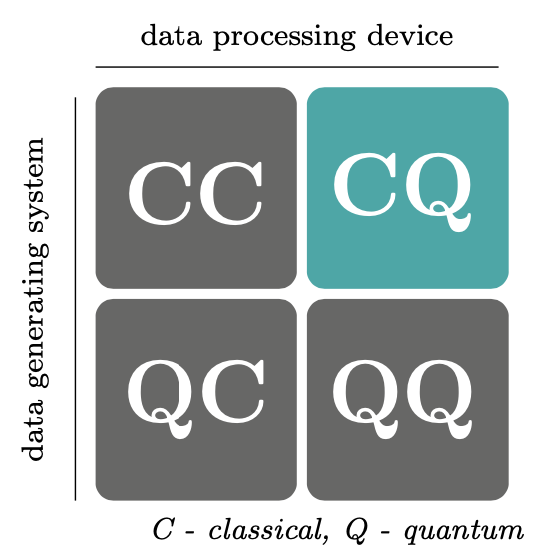
\includegraphics[keepaspectratio, scale=0.5]{introduction/4types.jpeg}
    \caption{4 types of quamtum machine learning.}
    \label{fig:4types}
\end{figure}

\par The idea of machine learning using quantum computers already existed at the dawn of quantum computers in the 1980s. The quantum model of neural networks was proposed in 1995 \cite{quest} and in 2000 \cite{assomem}. However, these studies were sporadic and did not attract enough attention to make quantum machine learning a major research topic. 

\par Quantum machine learning research has become popular just recently. Peter Wittek wrote a monograph \textit{Quantum Machine Learning— What quantum computing means to data mining} in 2014, which brought attention to quantum machine learning. Now quantum machine learning is one of the most vigorously studied fields in quantum computing research, and its research scope is wide-ranging.

\par The research of quantum machine learning can be divided into four types, which was proposed by Aimeur, Brassard and Gambs \cite{4types} (in Figure \ref{fig:4types}). These 4 types are divided by the assumptions whether the data is generated quantum (Q) or classically (C), and whether information is processed quantum (Q) or classically (C). 

\par CC means machine learning with classical data by using classical computers. CC is basically a conventional machine learning approach, but here it stands for machine learning that makes use of the knowledge of quantum computing. An example of the research of CC is \textit{tensor network} \cite{tensor1, tensor2}: tensor network is inspired by methods used to simulate quantum systems as efficiently as possible in classical computers, and now investigated for the purpose of processing high-dimensional data approximately in low-dimensional. 

\par QC means machine learning with quantum generated data by classical computations. QC is mainly aimed at simulating phenomena peculiar to quantum with classical computers. \cite{entannn,tomogra}

\par QQ means machine learning "quantum data" with the help of quantum computers. "Quantum data" is made up of quantum states generated by quantum computers, and after the generation directly used as the training dataset.

\par CQ means machine learning of classical data with the help of quantum computers. The classical data has to be encoded as a quantum state so that quantum computers are able to analyze it. 

\par This work focuses on supervised machine learning of classical data with the help of quantum computers, henceforth when we refer to quantum machine learning we mean CQ-type supervised machine learning.

\par Quantum-classical hybrid algorithms are said to be promising for quantum computing in the NISQ era when only approximate solutions can be obtained and the scale of quantum circuit executable is limited. Hybrid algorithms are widely used in quantum machine learning, and quantum devices are mainly used to produce the models, and classical computers fix those models to fit the given data.

\par There are two basic methods for quantum machine learning (sometimes used in other fields like quantum optimization, quantum eigenvalue solver, etc.), kernel method and variational method. These are quantum-classical hybrid algorithms, as mentioned earlier.
\section{Kernel method}
\par The problem we're targeting here is classification, one of the machine learning task to predict the label $y_i$ corresponding to the data $\bm{x_i}\in \mathbb{R}^m$, where $y_i \in \{1, -1\}$.
\par Assume the pairs of data and label $\{\bm{x_i, y_i}\}_{i=1,2,\cdots,N}$ where $\bm{x_i}\in \mathbf{R}^m$ is given. In order to improve the analysis performance, we consider nonlinear transformation of input data $\bm{x_i}$ to higher dimensional output $\hat{\bm{x_i}}$ as below.

$$\hat{\bm{x_i}}=\phi (\bm{x_i})\in \mathbf{R}^{\hat{m}}, \hat{m}>m$$

Then, we set the squared error cost function $f$ with parameters $\bm{w}\in\mathbb{R}^{\hat{m}}$ and by modifying these parameters we minimize the cost function. The cost function $f(\bm{w})$ is defined as below:

\begin{equation}
\label{heavy}
\begin{aligned}
f(\bm{w})=&\sum_{i=1}^N (y_i-\hat{\bm{x_i}}^{ \mathrm{T} }\bm{w})^2\\
=& \|\bm{y}-\bm{\hat{X}}\bm{w}\|^2_2
\end{aligned}
\end{equation}

where
$$\bm{y}=\{y_1,y_2,\cdots,y_N\}$$
$$\hat{\bm{X}}=(\hat{\bm{x_1}},\hat{\bm{x_2}},\cdots,\hat{\bm{x_N}})\in\mathbb{R}^{N\times \hat{m}}
$$
When $\hat{m}$ is large, computational cost to minimize the cost function $f$ increases.

\par On the other hand, if we can represent the parameters $\bm{w}$ with a linear combination of $\hat{\bm{x_i}}$, namely
$$\begin{aligned}
\bm{w}=&\sum_{i=1}^N \Tilde{w}\hat{\bm{x_i}}\\
=&\hat{\bm{X}}^{\mathrm{T}}\Tilde{\bm{w}}
\end{aligned}$$
where
$$\Tilde{\bm{w}}=(\Tilde{w_1},\Tilde{w_2},\cdots,\Tilde{w_N})^{\mathrm{T}}\in\mathbb{R}^N$$
then the cost function can be rewritten as below:
\begin{equation}
\label{ker}
\begin{aligned}
f(\Tilde{\bm{w}})&=\|\bm{y}-\hat{\bm{X}}\hat{\bm{X}}^{\mathrm{T}}\Tilde{\bm{w}}\|^2_2\\
&=\|\bm{y}-\bm{K}\Tilde{\bm{w}}\|^2_2\\
\end{aligned}
\end{equation}
where
$$\bm{K}=\hat{\bm{X}}\hat{\bm{X}}^{\mathrm{T}}=
\begin{pmatrix}
\hat{\bm{x_1}}^{\mathrm{T}}\hat{\bm{x_1}} & \hat{\bm{x_1}}^{\mathrm{T}}\hat{\bm{x_2}} & \hat{\bm{x_1}}^{\mathrm{T}}\hat{\bm{x_3}} & \cdots\\
\hat{\bm{x_2}}^{\mathrm{T}}\hat{\bm{x_1}} & \hat{\bm{x_2}}^{\mathrm{T}}\hat{\bm{x_2}} & & \\
\hat{\bm{x_3}}^{\mathrm{T}}\hat{\bm{x_1}} & & & \\
\vdots & & & \\
\end{pmatrix}\in\mathbb{R}^{N \times N}
$$
We write $ij$-th element of $\bm{K}$, namely $k_{ij}$ as $k(\bm{x_i},\bm{x_j})\ (=\hat{\bm{x_i}}^{\mathrm{T}}\hat{\bm{x_j}})$. The function $k$ is called as kernel function and the matrix $\bm{K}$ is called as kernel matrix.
If we can calculate the value of $k(\bm{x_i},\bm{x_j})$ efficiently, then the less computational cost to minimize the cost function \ref{ker} is achieved than \ref{heavy} due to the small dimension of the kernel matrix.

\par In the quantum kernel method, kernel function $k$ is calculated using the quantum circuit like Figure \ref{fig:kernel}. Minimization after calculating the kernel matrix is done on a classical computer.

\begin{figure}[H]
    \centering
    \Qcircuit @C=3.2em @R=1em {
        &&&\lstick{\ket{0}} & \multigate{4}{S(x)} & \multigate{4}{S(x')} & \meter  \\
        &&&\lstick{\ket{0}} & \ghost{S(x)} & \ghost{S(x')} & \meter \\
        &&&\lstick{\ket{0}} & \ghost{S(x)} & \ghost{S(x')} & \meter \\
        &&&\vdots & & &\vdots \\
        &&&\lstick{\ket{0}} & \ghost{S(x)} & \ghost{S(x')} & \meter
    }
    \caption{The circuit used for kernel method.\label{fig:kernel}}
\end{figure}

$S(\bm{x})$ is the unitary operation embedded the data $\bm{x}$ and can be freely defined.  $S(\bm{x'})\dagger$ is the inverse operation of $S(\bm{x'})$. Measurement is done by the measurement projector $|00\cdots0\rangle\langle00\cdots|$, which means the obtained value is the probability of all the qubits being in the state $|0\rangle$. The mathematical definition of kernel function $k$ is the following:
$$
\begin{aligned}
k(\bm{x},\bm{x'})&=\rm{tr} \left(|00\cdots 0\rangle\langle00\cdots 0|S(x')^\dagger S(x)|00\cdots 0\rangle \langle 00\cdots 0| S(x)^\dagger S(x')\right)\\
&=\|\langle 00\cdots 0|S(x')^\dagger S(x)|00\cdots 0\rangle\|^2\\
\end{aligned}$$

\par As seen from the above explanation, measurement of the quantum circuit on the order of $O(N^2)$ is needed with respect to the number of data $N$ to fill the elements of the kernel matrix. 
\section{Variational method}
\par The quantum circuit used in variational method is like Figure \ref{fig:variational}.

\begin{figure}[H]
    \Qcircuit @C=3.2em @R=1em {
        &&&\lstick{\ket{0}} & \multigate{4}{S(x)} & \multigate{4}{W(\theta)} & \meter  \\
        &&&\lstick{\ket{0}} & \ghost{S(x)} & \ghost{W(\theta)} & \meter \\
        &&&\lstick{\ket{0}} & \ghost{S(x)} & \ghost{W(\theta)} & \meter \\
        &&&\vdots & & &\vdots \\
        &&&\lstick{\ket{0}} & \ghost{S(x)} & \ghost{W(\theta)} & \meter
    }
    \caption{The circuit used for variational method.\label{fig:variational}}
\end{figure}

$S(\bm{x})$ is the unitary operation embedded with the data $\bm{x}$. This is the encoding operation and can be defined freely. $W(\bm{\theta})$ is the unitary operation embedded with some parameters and is the most important part of the variational method. $W(\bm{\theta})$ can be defined freely, and a pattern of $W(\bm{\theta})$ that determines which gates are applied to which qubits is called as ansatz. Measurement is done by the measurement operator $\mathcal{M}$.

\par This quantum circuit can be interpreted in two models: probabilistic models and  deterministic models. In the probabilistic models, measurement operator is selected so that the operator's eigenvalues correspond to the given label $y$, namely $\mathcal{M}=\sum y|y\rangle\langle y|$ where $\{|y\rangle\}$ is the orthonormal basis. Since $\sum|y\rangle\langle y|=I$ satisfies, 
$\tr\left(\mathcal{M}W(\theta)S(x)|00\cdots\rangle\langle00\cdots|S(x)^\dagger W(\theta)^\dagger\right)$ is equal to $1$ and the obtained value $\tr\left(|y\rangle\langle y|W(\theta)S(x)|00\cdots\rangle\langle00\cdots|S(x)^\dagger W(\theta)^\dagger\right)=|\langle y|W(\theta)S(x)|00\cdots\rangle|^2$ can be taken as the probability of the label of $x$ being $y$. Deterministic models are easier than the probabilistic models. We  construct the measurement operator $\mathcal{M}$ so that the measured value can directly be the output of the model.

\par In variational method, quantum circuits with parameters are used to produce models, and classical computers are used to adjust these parameters so that the models can represent the tendency of the given data. 

\par As can be seen in Figure \ref{fig:variational}, measurement of the quantum circuit on the order of $O(N)$ is needed with respect to the number of data $N$, which is more efficient than kernel method which needs $O(N^2)$ times measurement. Optimizers, which are algorithms of parameters adjustment, can be mainly divided into two directions: gradient-based algorithms and gradient-free algorithms.
\subsection{Optimizers}
\par Gradient-based algorithms utilize information from cost function gradients as like many classical machine learning algorithms that already exist. Parameters are basically updated in the direction opposite to the gradient value. The gradient of cost function can be analytically evaluated on quantum computers. There are two ways of evaluation: direct observation and indirect observation. Direct observation uses the auxiliary bit and the gradient is encoded into this bit, which means only one observable is needed \cite{Romero_2019}, while indirect observation can be implemented on the circuit of interest but requires multiple observables \cite{PhysRevResearch.1.013006}.

\par Gradient-free algorithm on the contrary does not need the evaluation of the gradient of the cost function. This algorithm takes advantage of the analytical properties of the cost function landscape. Therefore the design of the cost function is important for gradient-free algorithm. Few methods have been proposed:
Nelder-mead\cite{10.1093/comjnl/7.4.308}, Powell \cite{Pellow_Jarman_2021}, 
Rotosolve / Rotoselect \cite{Nakanishi_2020,Ostaszewski_2021}, Fraxis \cite{fraxis1,Wada_2022}, Quantum analytical descent \cite{koczor}.

\par What is important when using the variational method is that the cost function is tightly minimized and that parameters converge quickly. It is known that in quantum machine learning there can be a problem with the landscape of the cost function called barren plateaus, where the gradient is almost zero everywhere. This occurs especially when the number of parameters is increased in variational method with the gradient-based optimizer. However, gradient-free variational method directly jumps into an optimal solution, which prevents from getting stuck in barren plateaus \cite{book1}. From the convergence speed per iteration, gradient-free methods are also considered to be much faster than the gradient-based methods \cite{TILLY20221}. However, gradient-free optimizers use coordinate descent algorithms which update the parameters one by one, and require multiple (more thtaan three) expectation values to optimize one parameter. Gradient-based optimizers require only two expectation values, and are capable of optimizing all parameters at once. It may be unfair to compare the convergence speed per iteration between gradient-based optimizers and gradient-based optimizers, but several studies nonetheless show that in many cases the gradient-based optimizers converge faster\cite{Ostaszewski_2021,PhysRevResearch.2.043158, https://doi.org/10.48550/arxiv.1912.08660}.

\section{Our contributions}
\par Our aim is to make full use of exsitent quantum resources for machine learning with big data. In order to handle big data, it is necessary for the speed of training the model to be fast for the data size. Although  variational method is faster than kernel method, it is not sufficient when handling big data. In order to speed up variational method, we want to parallelize variational method with multiple quantum processors.
Furthermore, it is better if there is no need to aggregate given data to the central server, because communication of big data is troublesome (quantum federated learning).
  
\par In this paper, we propose a new distributed coordinate descent algorithm for quantum classification. 

\par Our research has impacts like below:

\begin{enumerate}
\item Our algorithm uses gradient-free optimizer for quantum machine learning, especially for classification. Up until now, algorithms using gradient-free optimizers are mainly focused on optimization problems or chemistry (solving eigenvalue problems for ground state energy computation), not with machine learning. We invent a new algorithm to construct a cost function for quantum classification, which makes it possible to minimize the function gradient-freely.

\item Our algorithm can be parallelized despite using a gradient-free optimizer. Up until now, distributed algorithms were based on gradient-based optimizers\cite{Qi_2022, 9775600}. This is thought to be due to the fact that gradient-free optimizers have not been considered for distributed quantum machine learning algorithms until now because gradient-based optimizers are very associated with classical machine learning. We invent distributed quantum machine learning algorithm using gradient-free optimizers, which are said to converge faster than gradient-based algorithms. This parallelization method makes it possible to do large-scale machine learning using big data.

\item Our algorithm achieves linear-scale speed up in training by the degree of parallelization. This feature is proved theoretically and also indicated by numerical simulations.

\item Our distributed algorithm behaves almost the same as the non-distributed one. Theoretically both behaviors are proved to be completely equal, and numerical simulations support this feature to some extent. Since the recently proposed distributed algorithms use gradient-based optimizers, the results obtained will inevitably change depending on the degree of parallelism. This is the drawback in these distributed algorithms, but we use gradient-free optimizer and that makes it possible to obtain the same result as the non-distributed one.
 \end{enumerate}

\begin{figure}[htb]
    \centering
    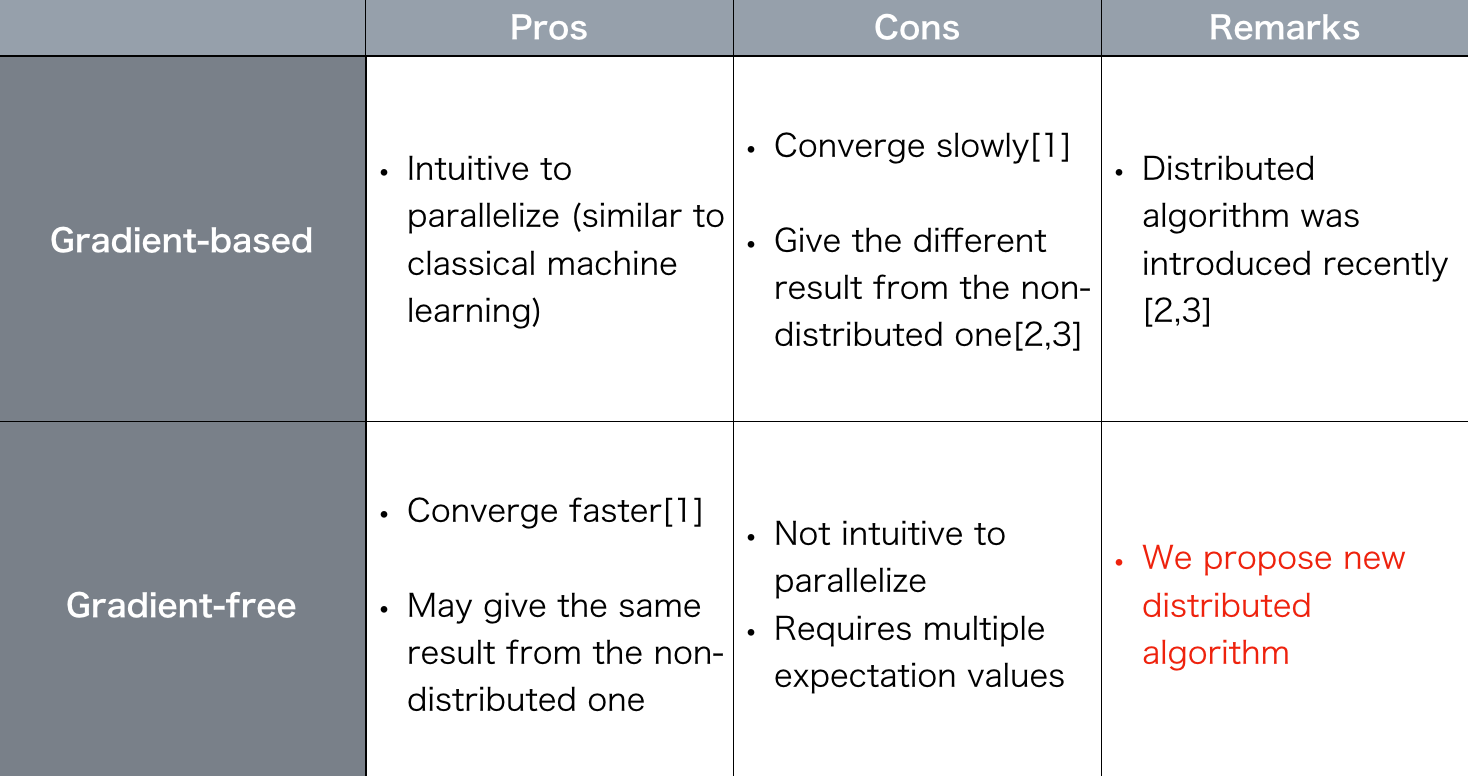
\includegraphics[keepaspectratio, scale=0.5]{introduction/optimizer.png}
    \caption{Our direction compared to the previous researches.}
    \label{fig:optimizer}
\end{figure}

%%%%%%%%%%%%%%%%%%%%%%%%%%%%%%%%%%%%%%%%%%%%%%%%%
%%%%%% preliminary
%%%%%%%%%%%%%%%%%%%%%%%%%%%%%%%%%%%%%%%%%%%%%%%%%

\chapter{Preliminary \label{chap:preliminary}}

\section{Notation}
\par $I, X, Y, Z$are the pauli matrices like below.
$$I=
\begin{pmatrix}
1 & 0\\
0 & 1\\
\end{pmatrix}$$
$$X=
\begin{pmatrix}
0 & 1\\
1 & 0\\
\end{pmatrix}$$
$$Y=
\begin{pmatrix}
0 & -i\\
i & 0\\
\end{pmatrix}$$
$$Z=
\begin{pmatrix}
1 & 0\\
0 & -1\\
\end{pmatrix}$$
\par Rotation operators $R_x, R_y, R_z$ are 1-qubit parameterized gates. These operators rotate the quantum state when considering the Bloch sphere by $\theta$ (parameter) about $X$ axis, $Y$ axis, $Z$ axis respectively. It is represented as follows using a matrix:

$$R_x(\theta)=\begin{pmatrix}
\cos{\theta} & -i\sin{\theta}\\
-i\sin{\theta} & \cos{\theta}\\
\end{pmatrix}$$

$$R_y(\theta)=\begin{pmatrix}
\cos{\theta} & -\sin{\theta}\\
\sin{\theta} & \cos{\theta}\\
\end{pmatrix}$$
$$R_z(\theta)=\begin{pmatrix}
\exp{\left(-i\frac{\theta}{2}\right)} & 0\\
0 & \exp{\left(i\frac{\theta}{2}\right)}\\
\end{pmatrix}$$

\par $\sqrt{X}$ gate is 1-qubit gate. If this gate is applied twice continuously on the qubit, the result is the same applying the x gate. Expressing this operation using a matrix gives:
$$\sqrt{X}=\frac{1}{2}
\begin{pmatrix}
1+i & 1-i\\
1-i & 1+i\\
\end{pmatrix}$$

\par CZ gate is the 2-qubits gate and works as a phase flipper for the target qubit if the control qubit is in $|1\rangle$. This gate is symmetric, that is, if the controled qubit and the target are exchanged, the result of the obtained quantum state is the same. Expressing this operation using a matrix gives:
$$
\begin{aligned}
CZ&=|0\rangle\langle0|\otimes I+|0\rangle\langle0|\otimes Z\\
&=\begin{pmatrix}
1 & 0 & 0 & 0\\
0 & 1 & 0 & 0\\
0 & 0 & 1 & 0\\
0 & 0 & 0 & -1\\
\end{pmatrix}
\end{aligned}$$

\begin{figure}[H]
    \centering
    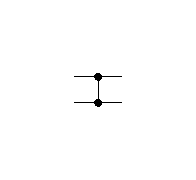
\includegraphics[keepaspectratio, scale=4]{preliminary/CZ.pdf}
    \caption{CZ gate is represented in the picture of quantum circuit like above.}
    \label{fig:CZ}
\end{figure}

\par Assume the $2\times 2$ unitary matrix $U$. When this matrix operation is applied to the $i$-th qubit of the circuit with $Q$ qubits, then $U_d$ is the unitary operation for circuit where the operation $U$ is applied to the $(d \mod Q)$-th qubit, and do nothing to any other qubits. Written as a formula, it looks like this:
$$U_d = I^{\otimes (e-1)}\otimes U\otimes I^{\otimes (Q-e)}$$
where
$$e = d\mod Q$$
\section{Fraxis gate}
\par Fraxis gate is the single qubit gate and can be defined as the $2\times 2$ unitary matrix $R(\bm{n})$ as the following,
$$\begin{aligned}
R(\bm{n})&=n_xX+n_yY+n_zZ
\end{aligned}$$
where $X$, $Y$, $Z$ are pauli matrices and parameters $\bm{n}=(n_x,n_y,n_x)^{ \mathrm{T} }$ satisfy the following :
$$\|\bm{n}\|^2=n_x^2+n_y^2+n_z^2=1
$$

\par Consider expressing one qubit quantum state on the Bloch sphere. It has been customary for a parameterized one-qubit gate to rotate the quantum state by a parameterized angle about some fixed axis. Fraxis gate breaks that convention and parameterizes the rotation axis by fixing the rotation angle to $\pi$ (See Figure \ref{fig:gate}).

On actual quantum processors, the number of quantum gates that can be used is limited, and various unitary operations are performed by combining gates available. Fraxis gate has to be also performed by those basic gates. For example, on ibmq\_montreal, fraxis gate is implemented as follows:
$$R(\bm{n})=R_z(\phi+\pi)\cdot\sqrt{X}\cdot R_z(\theta+\pi)\sqrt{X}\cdot R_z(\pi-\phi)$$
where
$$\theta=2\arctan\left(\frac{\sqrt{n_x^2+n_y^2}}{n_z}\right)$$
$$\phi=\arctan\left(\frac{n_y}{n_x}\right)$$

\begin{figure}[H]
    \centering
    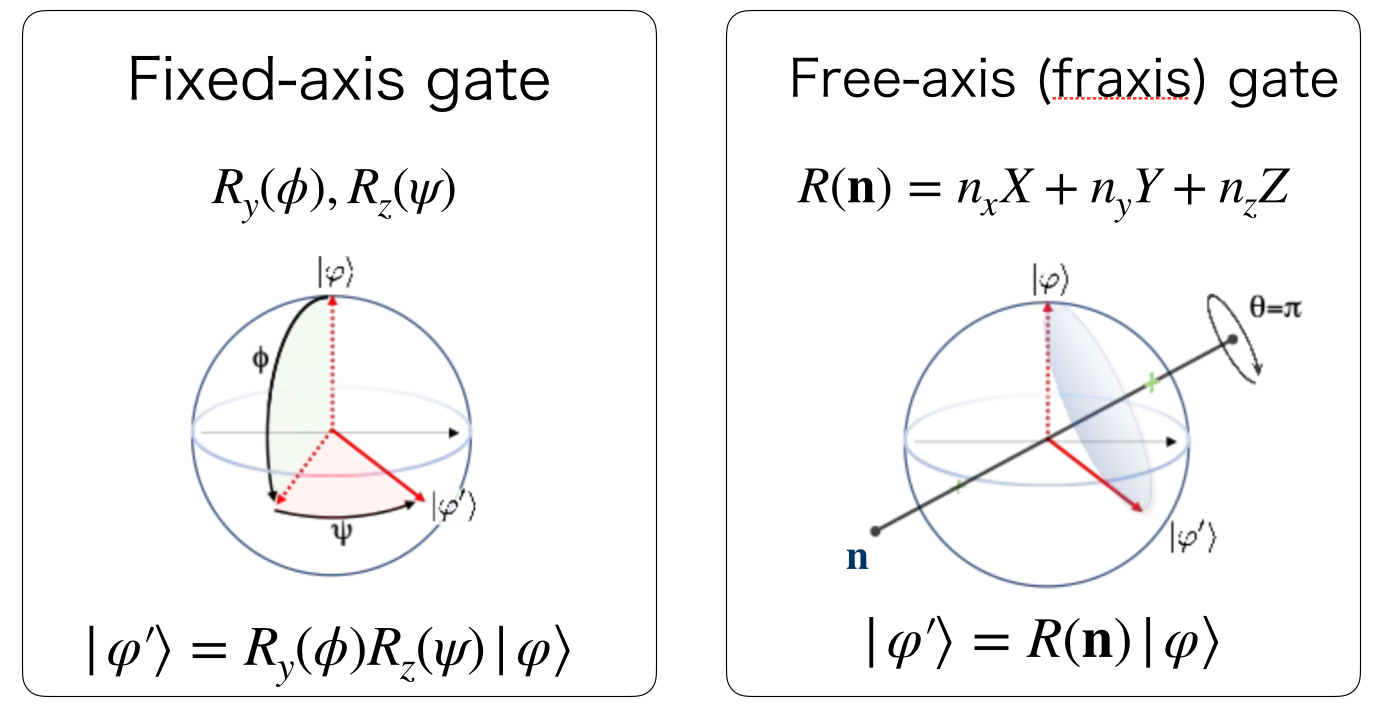
\includegraphics[keepaspectratio, scale=0.5]{preliminary/gate.png}
    \caption{Comparison of fraxis gate with the traditional parameterized gate. The pictures show how to rotate the quantum state $|\varphi\rangle$ to $|\varphi'\rangle$.}
    \label{fig:gate}
\end{figure}
\section{Data encoding}
\par In this work, we focus on CQ, which means machine learning of classical data with quantum devices. Therefore, we need to encode the classical data into some  quantum state. A properly chosen encoding method can greatly improve the accuracy of machine learning. In quantum machine learning, sometimes encoding data is the bottleneck for the runtime of the algorithm. 

\subsection{Amplitude encoding}
\par Assume that the data $\bm{x}$ is the $2^Q$-dimensional real vector. Then, the representation of this data is the following:
$$|\psi\rangle=\sum_{k=1}^{2^Q}\frac{x_k}{\|\bm{x}\|}|k\rangle$$
where $x_k$ is the k-th element of $\bm{x}$, and $\|.\|$ is the L2-norm. The number of the required qubits is $Q$.

\par The problem of amplitude encoding is that it takes much time to prepare the quantum state. It is known that the lower bound of circuit depth for amplitude encoding is $O\left(\frac{2^Q}{Q}\right)$ for circuit with $Q$ qubits \cite{lower}. The actual algorithm currently used is worse than this and takes almost $O(2^N)$ circuit depth \cite{book1}.

\subsection{Angle encoding}
\par Assume that the data $\bm{x}$ is the $LQ$-dimensional real vector. The representation of this data is done for example by the following circuit (Figure \ref{fig:circuit5}). The number of the required qubits is $Q$. 
\begin{figure}[htb]
    \centering
    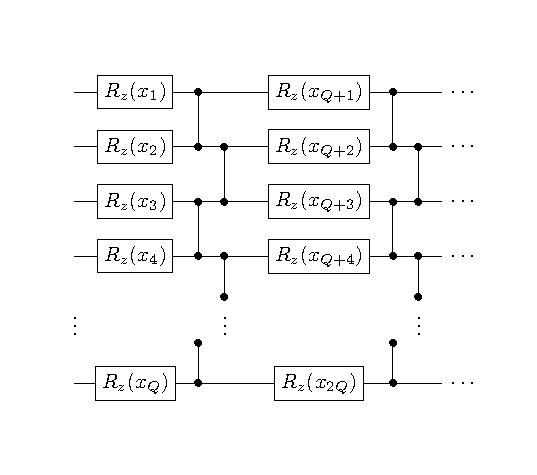
\includegraphics[keepaspectratio, scale=2]{preliminary/angle_enco.pdf}
    \caption{The example circuit of angle encoding for $LQ$-dimensional data.}
    \label{fig:circuit5}
\end{figure}

\par In this example, the first $Q$ elements are embedded into each qubit using $R_z$ gates, then these qubits are entangled using a CZ layer, and the next $Q$ elements are embedded into each qubit using fraxis gates, then entangle these qubits using a CZ layer, and so on $L$ times. Rotation operators can be $R_y$ or $R_z$. The order of data, the number of qubits, etc. can be freely determined. A method of encoding using a rotating game is called angle encoding.It is clear that the circuit depth is $O(N)$ for the data $\bm{x}\in\mathbb{R}^N$, which is far shallower than amplitude encoding.


%%%%%%%%%%%%%%%%%%%%%%%%%%%%%%%%%%%%%%%%%%%%%%%%%
%%%%%% method
%%%%%%%%%%%%%%%%%%%%%%%%%%%%%%%%%%%%%%%%%%%%%%%%%

\chapter{Method \label{chap:method}}

\section{Optimization scheme}
\par Again, we clarify the problem setting. We have dataset which is pair of data and label  $\{(\bm{x^{(i)}}, y^{(i)})\}_{i=1,2,\cdots,N}$, where  $y^{(i)}\in\{-1,1\}$. By learning this dataset, we hope to be able to predict suitable labels for unlabeled data. 

\par Assume that we have the following circuit in Figure \ref{fig:abst1}.
\begin{figure}[htb]
    \centering
    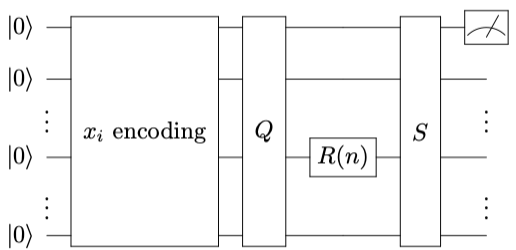
\includegraphics[keepaspectratio, scale=1.5]{method/abst1.png}
    \caption{The fraxis gate that we are interested in and want to optimize is expressed explicitly.}
    \label{fig:abst1}
\end{figure}
Here, $Q$ and $S$ are the unitary operations. Fraxis gate $R(\bm{n})$ is applied to the $d$-th qubit. As seen in Figure \ref{fig:abst1}, the first qubit is measured by observable $Z$ and its value ranges from -1 to 1. This value can be written as following:
$$\upsilon_i=\tr{\left(Z_1 SR_d(\bm{n})Q\rho_{i} Q^\dagger R_d(\bm{n})^{\dagger}S^\dagger\right)}$$
We call this value as $\upsilon_i$ and define it as the prediction value of the label by the quantum circuit in Figure \ref{fig:abst1}. That means:
$$y_i \longleftarrow
\left\{
\begin{array}{ll}
-1 & \ \ \rm{if}\ \upsilon_i<0\\
1 & \ \ \rm{otherwise}\\
\end{array}
\right.
$$

\par Then, we define the cost function like below:
$$-\sum_{i=1}^N y_{i}\upsilon_i$$
Intuitively, when the predicted value and the actual label match, the value of the cost function is reduced, and vice versa.

\par Our method for minimizing the cost function is described below. First, we transform the cost function and see that the cost function can be written in a very simple form. For simplicity of notation, we write $Q\rho_i Q^\dagger$ as $\rho_i$, and $S^\dagger Z_1 S$ as $\mathcal{M}$.
$$
\begin{aligned}
&-\sum_{i=1}^Ny_i\upsilon_i\\
=&-\sum_{i=1}^N y_{i}\tr(\mathcal{M} R(\bm{n}){\rho_{i}}R(\bm{n}^\dagger)\\
=&-\sum_{i=1}^N y_{i} (n_{x}^2\tr(\mathcal{M} X\rho_{i} X)+n_{y}^2\tr(\mathcal{M} Y\rho_{i} Y)+n_{z}^2\tr(\mathcal{M} Z\rho_{i} Z)\\
&+n_{x}n_{y}\tr(\mathcal{M} X\rho_{i} Y+\mathcal{M} Y\rho_{i} X)\\
&+n_{y}n_{z}\tr(\mathcal{M} Y\rho_{i} Z+\mathcal{M} Z\rho_{i}Y)\\
&+n_{z}n_{x}\tr(\mathcal{M} Z\rho_{i} X+\mathcal{M} X\rho_{i} Z))\\
=&-\sum_{i=1}^N y_{i}(n_{x}^2 g_{ix} + n_{y}^2 g_{iy} + n_{z}^2 g_{iz}\\
&+n_{x}n_{y}(2g_{ixy}-g_{ix}-g_{iy})+n_{y}n_{z}(2g_{ixz}-g_{iy}-g_{iz})+n_{z}n_{x}(2g_{iz}-g_{ix}-g_{iz}))\\
=&-\sum_{i=1}^N y_{n}\bm{n}^\top G_{i} \bm{n}\\
=&-\bm{n}^\top\left(\sum_{i=1}^N  y_{n}G_{i}\right)\bm{n}\\
=&-\bm{n}^\top G \bm{n}\\
\end{aligned}
$$
where 
$$
\begin{aligned}
g_{ix}&=\tr(\mathcal{M} X\rho_{i}X)\\
g_{iy}&=\tr(\mathcal{M} Y\rho_{i}Y)\\
g_{iz}&=\tr(\mathcal{M} Z\rho_{i}Z)\\
g_{ixy}&=\tr(\mathcal{M} \frac{X+Y}{\sqrt{2}}\rho_{i}\frac{X+Y}{\sqrt{2}})\\
g_{ixz}&=\tr(\mathcal{M} \frac{X+Z}{\sqrt{2}}\rho_{i}\frac{X+Z}{\sqrt{2}})\\
g_{iyz}&=\tr(\mathcal{M} \frac{Y+Z}{\sqrt{2}}\rho_{i}\frac{Y+Z}{\sqrt{2}})\\
\end{aligned}$$
and
$$G_{i}=
\begin{pmatrix}
g_{ix} & g_{ixy}-\frac{g_{ix}+g_{iy}}{2} & g_{ixz}-\frac{g_{ix}+g_{iz}}{2}\\
g_{ixy}-\frac{g_{ix}+g_{iy}}{2} & g_{iy} & g_{iyz}-\frac{g_{iy}+g_{iz}}{2}\\
g_{ixz}-\frac{g_{ix}+g_{iz}}{2} & g_{iyz}-\frac{g_{iy}+g_{iz}}{2} & g_{iz}\\
\end{pmatrix}
$$
\par All the elements of $G_i$, that means $g_x, g_y, g_z, g_{xy}, g_{xz}, g_{yz}$, is obtained by replacing the fraxis gate $R(\bm{n})$ we focus on now. Therefore, in order to construct the matrix $G$, 6 observations of the quantum circuit are required for every data $\{x_i\}\ (i=1,2,\cdots, N)$.
\par Note, that 
$$G=\sum_{i=1}^N  y_{i}G_{i}$$
is the real symmetric matrix. By the following theorem, the optimal value to minimize the cost function is the maximum eigenvalue of this real symmetric matrix $G$.

\subsubsection{Theorem}
When the matrix $G=\sum_{i=1}^Ny_iG_i$ has eigenvalues $\lambda_1 \leq \lambda_2 \leq \lambda_3$ (corresponding
eigenvectors as $n_1, n_2, n_3$, $\|n_1\|= \|n_2\| = \|n_3\| = 1$), then the followings holds.
$$\argmax_{\|n\|=1} n^\top Gn = n_3$$
$$\max_{\|n\|=1} n^\top Gn = \lambda_3$$
\subsubsection{Proof}
We define the function $f$ and $\hat{\bm{n}}$:
$$f(n,\tau)=n^\top Gn-\tau(\|n\|^2-1)$$
$$\hat{n} = \argmax_{\|n\|=1} n^\top Gn$$

By the method of Lagrange multipliers, at the point $\hat{n}$, there exists 
$\hat{\tau}$ that satisfies the following.
$$\frac{\partial f}{\partial n}(\hat{n}, \hat{\tau} ) = 0$$
By solving these equations, we get
$$2G \hat{n} = \hat{\tau} \hat{n}$$
Here we use the formula $\frac{\partial }{\partial \bm{x}}\bm{x}^\top A\bm{x}=(A+A^\top)\bm{x}$ (see \ref{chap:appendix}).

\par Therefore, $\hat{n}$ is one of the eigenvectors of $G$, $n_1, n_2, n_3$.
Since 
$$\begin{aligned}
n_k^\top Gn_k&=\lambda_kn_k^\top n_k\\
&=\lambda_k\|n_k\|^2_2\\
&=\lambda_k
\end{aligned}$$
holds, from the condtion $\lambda_1\leq\lambda_2\leq\lambda_3$  directory follows $\hat{n}=n_3$.
\\
\\
\\
The discussion so far can be summarized as follows. Assume the quantum circuit to calculate the cost function has one fraxis gate we are now focusing on. We replace this fraxis gate with $X, Y, Z, \frac{X+Y}{\sqrt2}, \frac{X+Z}{\sqrt2}, \frac{Y+Z}{\sqrt2}$, and calculate the value obtained from the replaced quantum circuit for every data. For each data, we construct the matrix $G_i$, and sum up all $G_i$ with the label $y_i$. Finally we get the symmetric matrix $G$, next solve the eigenvector of $G$ which corresponds to the maximum eigenvalue of $G$. This eigenvector is the optimal parameters for the fraxis gate we are focusing now on. The operation of applying the above operations to all the gates included in the quantum circuit is repeated.
\section{Parallelization on multiple qunatum devices}
As seen above, minimization of the cost function can be returned to solving the eigenvalues of matrix $G=\sum_{i=1}^Ny_iG_i$, where $N$ is the data size. 
Here, let the data size be $N$ times $M$ again, and consider obtaining the matrix $G$. If $G^{(m)}$ is newly defined as follows, 
$$G^{(m)}=\sum_{i=(m-1)N+1}^{mN}y_iG_i$$
G can be written as $G=\sum_{m=1}^MG^{(m)}$. Thus, if there are $M$ quantum devices, it is possible that $NM$ pieces of data are divided into $M$ equal parts and sent to quantum devices by $N$ pieces, each device calculates $G^{(m)}$, sends the calculation result to the central server, and the central server adds all the matrix $G^{(m)}$ sent to itself to obtain $G$. As can be seen from the above, unlike the gradient-based optimizer \cite{9775600, Qi_2022}, parallelization of this algorithm does not change the progress of learning. Parameters are optimized exactly the same as without parallelization.

\begin{figure}[htb]
    \centering
    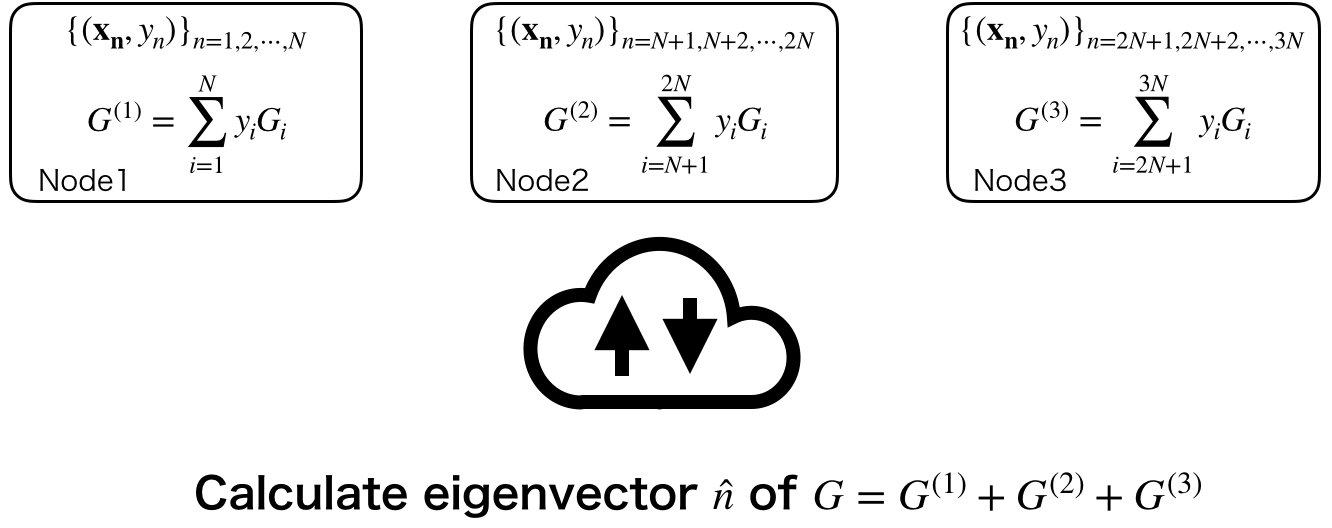
\includegraphics[keepaspectratio, scale=0.5]{method/example.png}
    \caption{Example of parallelization by 3 quantum nodes.}
    \label{fig:example}
\end{figure}
\section{Algorithm}
\par From the discussion above, when there is one fraxis gate in the circuit, we know how to parallelize and optimize the parameters in that gate. However, there are multiple fraxis gates in the circuit and it is difficult to optimize all of them perfectly. Therefore, we propose to use a coordinate descent algorithm in order to approximately optimize this circuit when there are multiple fraxis gates. In the coordinate descent method, each fraxis gate is focused on in turn, and it is repeated to fix the parameters of the remaining non-focused gates and optimize only the parameters of the focused gate as described as mentioned in previous sections.

\par The overall optimization algorithm is shown below:

\begin{figure}[htb]
\begin{algorithm}[H]
\label{alg:algdis}
  \begin{algorithmic}[1]
    \caption{Circuit optimization for classification with free-axis selection}
        \Require $M$ local quantum circuits for classification, Number of fraxis gates L, central server, initialized parameters $\{\bm{n_i}\}_{i=1,2,\cdots,L}$ (satisfies $\|\bm{n_i}\|=1$), data and label $\{(\bm{x_{i}}, y_i)\}_{i = 1, 2, \cdots, N}$, and \# repetitions $T$
        \Ensure optimized parameters of $\{\bm{n_i}\}_{i=1,2,\cdots,L}$
        \State Divides the data and labels equally for $M$ local nodes
        \For{$t$ in $t=1,2,\cdots,T$}
            \For{$d$ in $d=1,2,\cdots,L$}
                \State $G \longleftarrow \bm{0}$
                \For{$m$ in $m=1,2,\cdots,M$ \textbf{in parallel}}
                    \State $G^{(m)} \longleftarrow \bm{0}$
                        \For{$i$ in $i=1,2,\cdots, \frac{N}{M}$}
                            \State Computes $G_i$
                            \State $G^{(m)} \longleftarrow G^{(m)}+ y_iG_i$ 
                        \EndFor
                    \State $G\longleftarrow G+G^{(m)}$ 
                \EndFor
                \State Computes the eigenvector $\bm{\hat{n_d}}$ of the maximum eigenvalue of $G$
                \State $\bm{n_d} \longleftarrow \bm{\hat{n_d}}$
            \EndFor
        \EndFor
        \State \Return $\{\bm{n_i}\}_{i=1,2,\cdots,L}$
  \end{algorithmic}
  \end{algorithm}
\end{figure}

Looking at the algorithm above, it is clear that the order of execution time is $O(\frac{NLT}{M})$, where $N$ is the data size, $L$ is the number of fraxis gates, $T$ is the number of times to update all fraxis gates and $M$ is the number of quantum local nodes, which means the degree of parallelization. It is shown that the execution time can be reduced in inverse proportion to $M$ by $M$-parallelism.

%%%%%%%%%%%%%%%%%%%%%%%%%%%%%%%%%%%%%%%%%%%%%%%%%
%%%%%% experiments
%%%%%%%%%%%%%%%%%%%%%%%%%%%%%%%%%%%%%%%%%%%%%%%%%

\chapter{Experiments on simulator \label{chap:experiments}}
\par In this chapter, we show the experiments of numerical simulation of image classification. This simulation is implemented with Python, and the main libraries used are NumPy \cite{harris2020array} for solving eigenvalue / eigenvector, Qiskit \cite{Qiskit} for quantum circuit simulator, PyTorch \cite{NEURIPS2019_9015} for parallelization. The experiments were conducted on Intel(R) Core(TM) i7-8750H CPU @ 2.20GHz 2.21GHz. The code used in this chapter is available from \cite{mycode}.
\section{Data}
\par We conducted image classification experiments by using MNIST \cite{lecun-mnisthandwrittendigit-2010} and Fashion-MNIST dataset \cite{xiao2017fashionmnist}. 

\par MNIST is the database of $28\times28$ pixel grayscale images of handwritten digits from 0 to 9. From this dataset, we select the data labeled 0 or 1 for binary classification and make a new dataset. The data 0 have been relabeled as 1 and the data 1 have been relabeled as -1. This dataset consists of 12,665 training images (6,742 images are labeled as 1) and 2,115 evaluation images (1,135 images are labeled as 1). 

\par Fashion-MNIST is the database of $28\times28$ pixel grayscale images of 10 types of fashion products,  T-shirt/top, trouser, pullover, dress, coat, sandal, shirt, sneaker, bag, ankle boot. Labels are assigned from 0 to 9 in this order. From this dataset, we select the data labeled 0 or 1 for binary classification and make a new dataset. The data 0 have been relabeled as 1 and the data 1 have been relabeled as -1. This dataset consists of 12,000 training images (6,000 images are labeled as 1) and 2,000 evaluation images (1,000 images are labeled as 1).

\begin{figure}[htb]
    \centering
    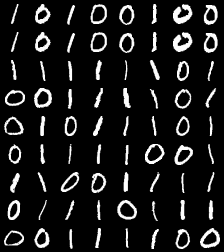
\includegraphics[keepaspectratio, scale=0.5]{experiment/figure/mnist.png}
    \caption{Some images of MNIST labeled with 0 and 1.}
    \label{fig:mnist}
\end{figure}

\begin{figure}[htb]
    \centering
    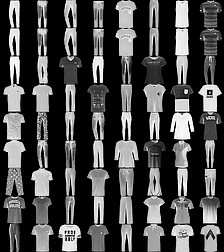
\includegraphics[keepaspectratio, scale=0.5]{experiment/figure/fmnist.png}
    \caption{Some images of Fashion-MNIST labeled with 0 (T-shirt/top) and 1 (trouser).}
    \label{fig:fmnist}
\end{figure}

\par These images have too many pixels, so we reduce them to $8\times8$ pixel images by setting the resize method of the OpenCV library with the interpolation method set to inter\_area \cite{opencv_library}. After that, they are flattened by converting it to a $64$-dimensional vectors and normalized.
\section{Circuit}
\subsection{Data encoding}
\par In this experiment, we use fraxis encoding. Fraxis encoding is newly introduced in this research, and is very similar to angle encoding.

\subsubsection{Fraxis encoding}
\par Assume that the data $\bm{x}$ is the $2LQ$-dimensional real vector. Then, the representation of this data is done by the following circuit (Figure \ref{fig:fraxis_enco}). The number of the required qubits is $Q$. 

\begin{figure}[H]
    \centering
    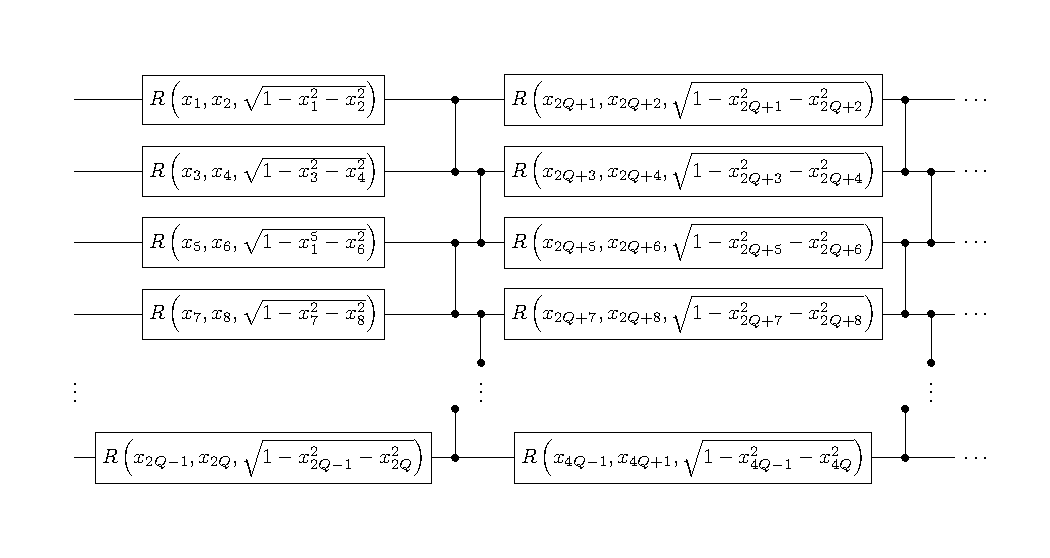
\includegraphics[keepaspectratio, scale=0.5]{experiment/figure/fraxis_enco.pdf}
    \caption{Fraxis encoding used in this research.}
    \label{fig:fraxis_enco}
\end{figure}

\par As seen above, the first $2Q$ elements are embedded into each qubit using fraxis gates, then these qubits are entangled using a CZ layer, and the next $2Q$ elements are embedded into each qubit using fraxis gates, then entangle these qubits using a CZ layer, and so on $L$ times. When the dimension of the data is not $2LQ$, we place elements from the beginning into the fraxis encoding, and the remaining elements are put in fraxis gate's parameters and appended to the end of fraxis encoding.

\subsection{Overall circuit}
Here we define the fraxis layer as shown in Figure \ref{fig:ansatz}.
\begin{figure}[H]
    \centering
    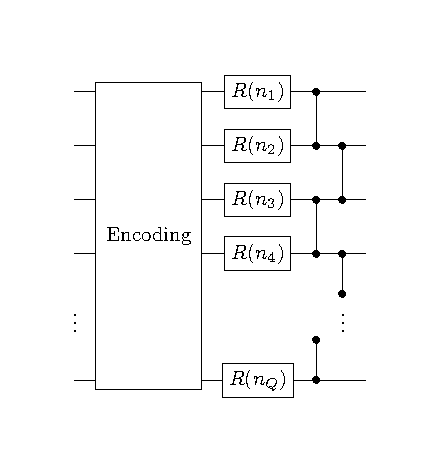
\includegraphics[keepaspectratio, scale=1]{experiment/figure/layer.pdf}
    \caption{Fraxis layer on $Q$ qubits.}
    \label{fig:ansatz}
\end{figure}
After encoding the data, fraxis gates is applied to all bits and finally CZ gates are alternately applied.
\par The entire circuit repeats this fraxis layer $L$ times, as shown in the figure \ref{fig:whole}.
\begin{figure}[H]
    \centering
    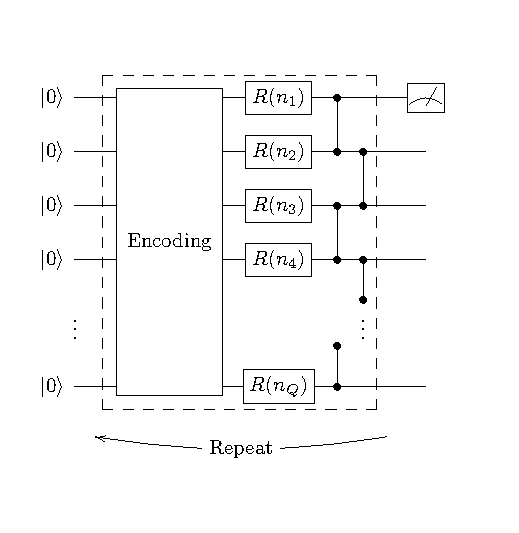
\includegraphics[keepaspectratio, scale=1]{experiment/figure/whole.pdf}
    \caption{Overall circuit on $Q$ qubits.}
    \label{fig:whole}
\end{figure}

\par In this experiments, we initialize all the fraxis gates' parameters to $\bm{n}=(0,0,1)^\top$. The order of the updating of the parameters are cyclically fixed. That means, from the fraxis gate of the first qubit of the first layer, then the second qubit of the first layer, and so on to the final qubit of the first layer, and after the updating of the first layer, then the second layer, the third layer, and so on.
\section{Results}
In the following, we introduce the experimental results  of numerical simulation. 
\subsection{Change the number of qubits}
Here, we show how the variational quantum circuit converges when the number of fraxis ansatz is fixed at 3 and the number of qubits is changed from 2 to 8. The number of training data and evaluation data sizes are both fixed at 100.

\begin{figure}[H]
    \centering
    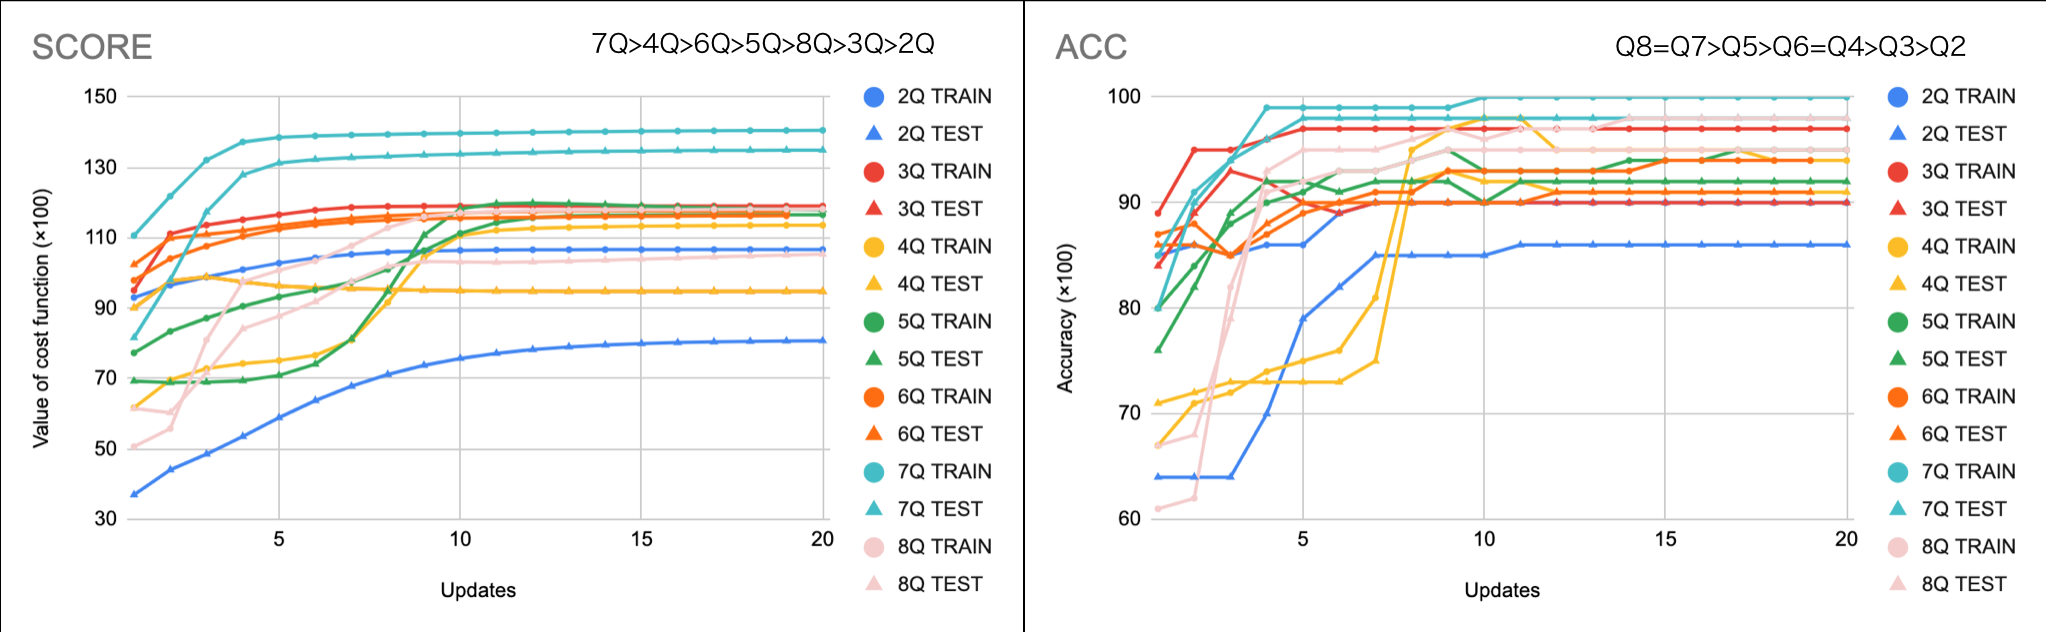
\includegraphics[keepaspectratio, scale=0.43]{experiment/figure/MNIST_qubit_change.png}
    \caption{MNIST classification with changed number of qubits. Fixed at 3 fraxis layers, 100 training and evaluation data.}
    \label{fig:MNIST_qubit_change}
\end{figure}
\begin{figure}[H]
    \centering
    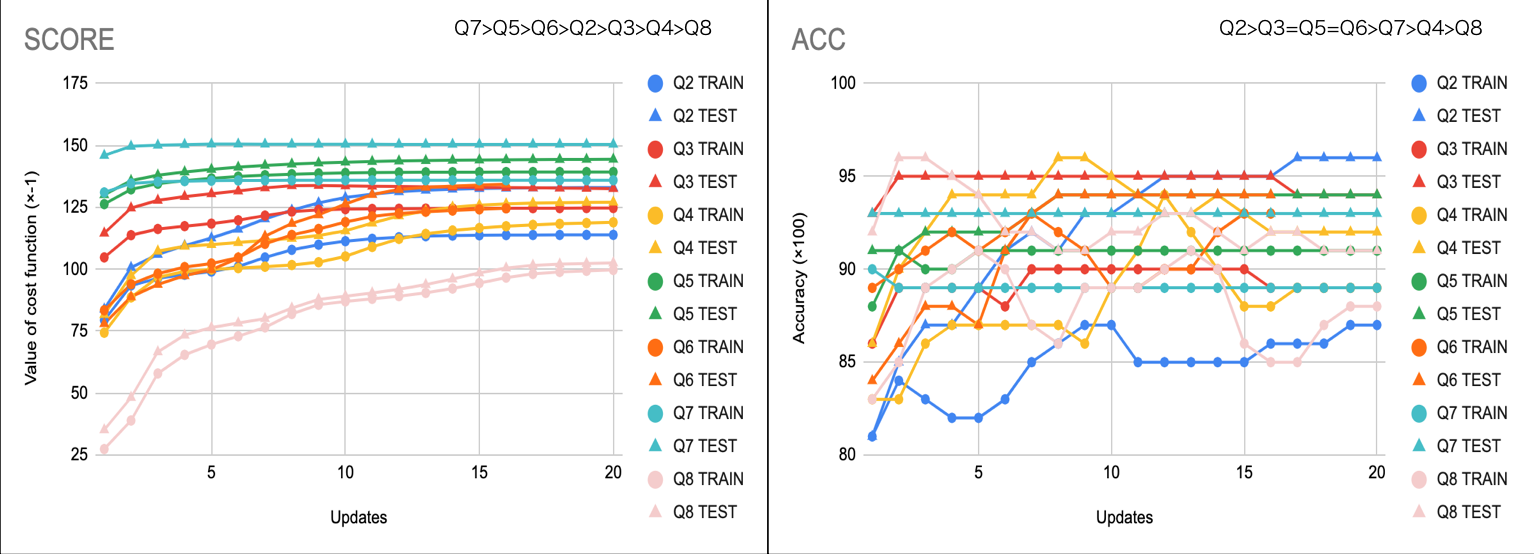
\includegraphics[keepaspectratio, scale=0.57]{experiment/figure/FMNIST_qubit_change.png}
    \caption{Fashioon-MNIST classification with changed number of qubits. Fixed at 3 fraxis layers, 100 training and evaluation data.}
    \label{fig:FMNIST_qubit_change}
\end{figure}

\par Figure \ref{fig:MNIST_qubit_change} indicates that more qubits result better, on the other hand, Figure \ref{fig:FMNIST_qubit_change} indicates the contrary. Generally speaking, more qubits result in more expressibility of the quantum circuit, so the quantum circuit with the more number of qubits should perform better than the circuit with less qubits. The results of \ref{fig:FMNIST_qubit_change} contradict this. It is thought that the increase in qubits (that is, the increase in fraxis gates, or the parameters to be optimized) made optimization difficult. In addition, even though training progresses, a temporary decrease in accuracy is observed.\\

\subsection{Change the number of fraxis layer}
Here, we show how the quantum circuit converges when the number of qubits is fixed at 2 and the number of fraxis layer is changed from 1 to 3. The number of the training data and the evaluation data are both fixed at 100. 

\begin{figure}[H]
    \centering
    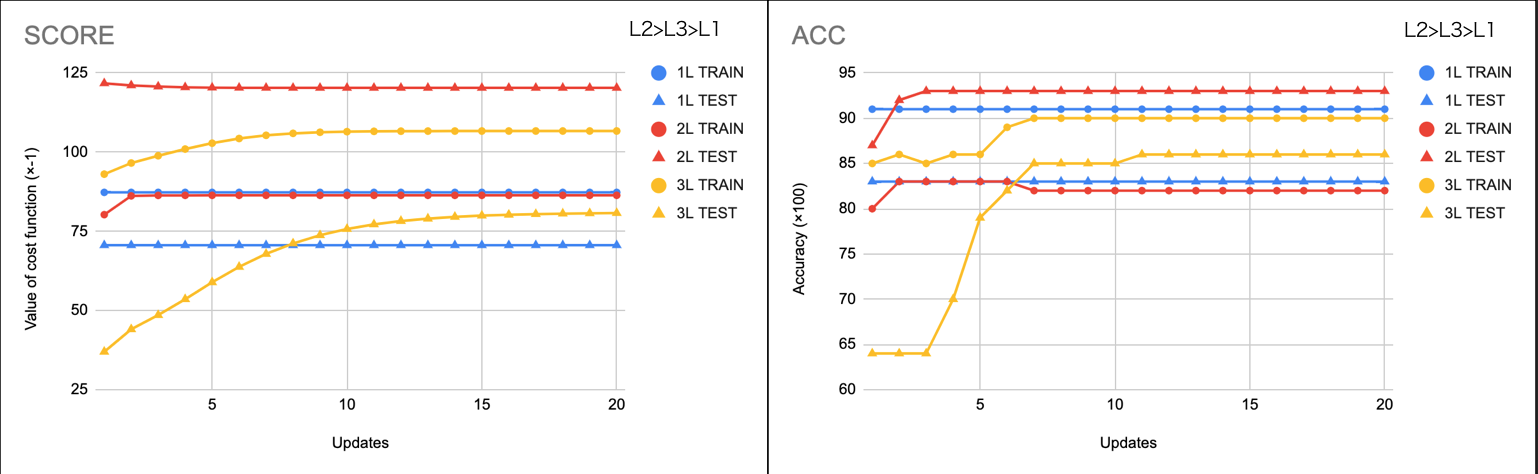
\includegraphics[keepaspectratio, scale=0.54]{experiment/figure/MNIST_layer_change.png}
    \caption{MNIST classification with changed number of fraxis layer. Fixed at 2 qubits, 100 training and evaluation data.}
    \label{fig:MNIST_layer_change}
\end{figure}
\begin{figure}[H]
    \centering
    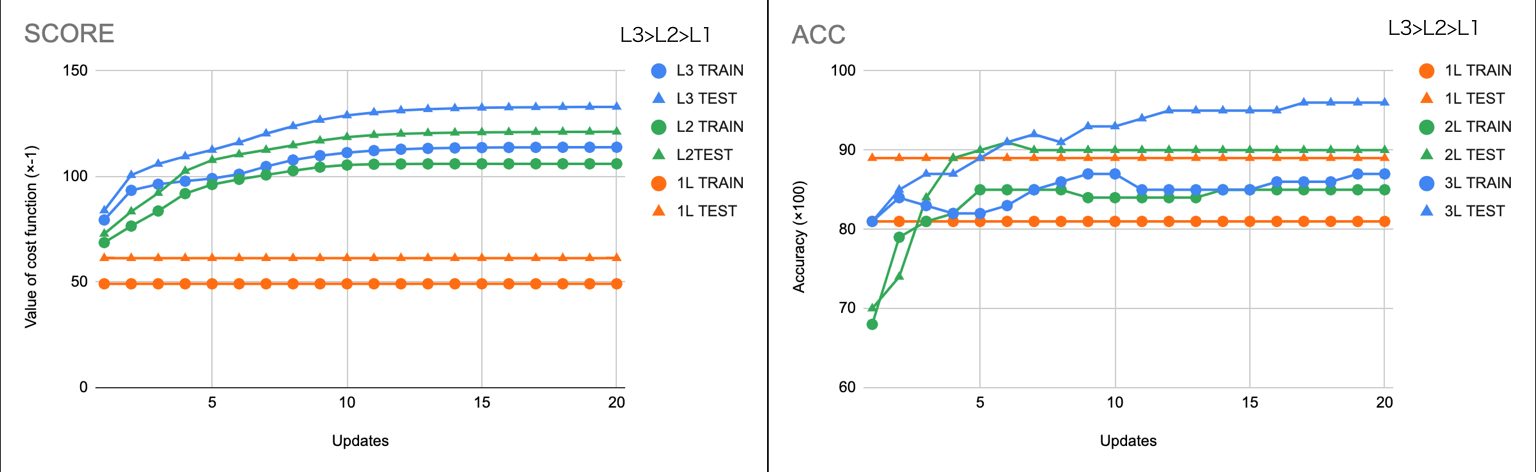
\includegraphics[keepaspectratio, scale=0.54]{experiment/figure/FMNIST_layer_change.png}
    \caption{Fashioon-MNIST classification with changed number of fraxis layer. Fixed at 2 qubits, 100 training and evaluation data.}
    \label{fig:FMNIST_layer_change}
\end{figure}

\par Figure \ref{fig:FMNIST_layer_change} indicates that more fraxis layers result better, on the other hand, Figure \ref{fig:MNIST_layer_change} indicates that more fraxis layer does not necessarily mean the better result. More layers mean the more parameters to be optimized, therefore, in general, result in better performance. The results of \ref{fig:MNIST_layer_change} do not follow this. It is thought that the increase in fraxis layers (that is, the increase in fraxis gates, or the parameters to be optimized) made optimization difficult. In addition, even though training progresses, a temporary decrease in accuracy is observed.\\

\subsection{Change the degree of parallelization}
Here we show how our algorithm can achieve the parallelization. We change the number of quantum nodes ny simulation from 1 to 3. The number of the training data and the evaluation data are both fixed at 100, the number of qubit is 6, and the number of fraxis layer is 3. The MNIST dataset is used.
\begin{figure}[H]
    \centering
    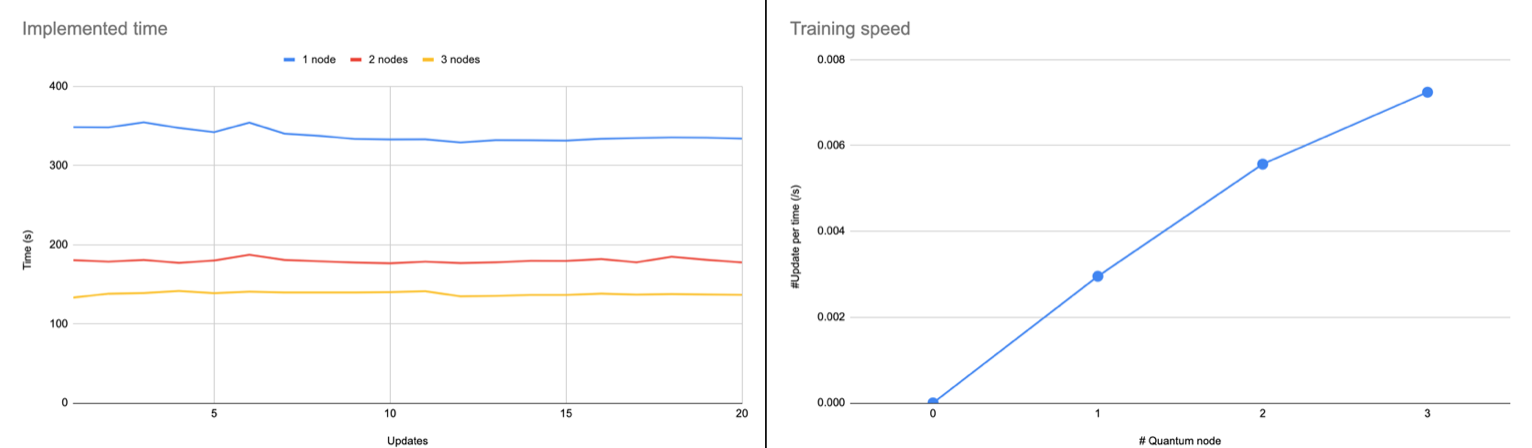
\includegraphics[keepaspectratio, scale=0.54]{experiment/figure/MNIST_node_change_time.png}
    \caption{MNIST classification with changed number of the quantum node. Fixed at 6 qubits, 3 fraxis layers, 100 training and evaluation data.}
    \label{fig:MNIST_node_change_time}
\end{figure}
\begin{figure}[H]
    \centering
    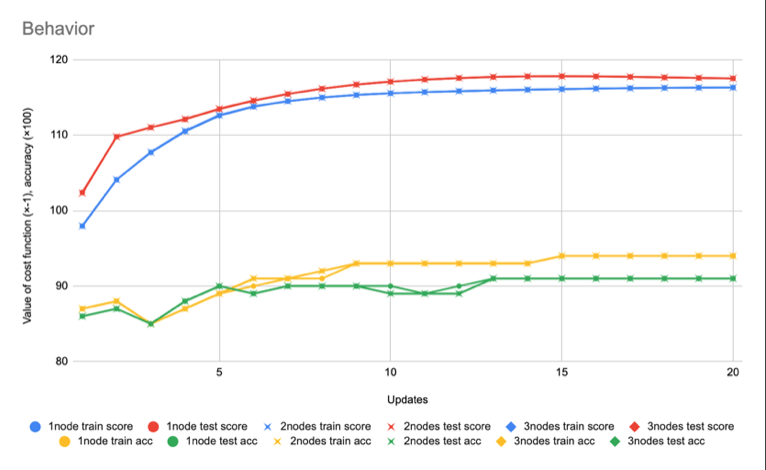
\includegraphics[keepaspectratio, scale=0.54]{experiment/figure/MNIST_node_change_behavior.png}
    \caption{MNIST classification with changed number of the quantum node. Fixed at 6 qubits, 3 fraxis layers, 100 training and evaluation data.}
    \label{fig:MNIST_layer_change_behavior}
\end{figure}

\par Figure \ref{fig:MNIST_node_change_time} indicates the parallelization achieves the speed up the training in almost linear-scale as shown theoretically above. Figure \ref{fig:MNIST_layer_change_behavior} indicates that the parallelization makes little change in behavior, but theoretically behavior of distributed algorithms (in which the number of quantum nodes is two or three) must completely match behavior of non-distributed one (in which the number of quantum nodes is one). These differences in behavior of algorithms is caused by precision loss. Our proposed parallelization scheme changes the order of addition (subtraction) calculations when aggregating and summing up the matrix $G^{(i)}$ to construct the matrix $G$. This change of the calculation order produces precision loss and minor differences between distributed algorithm and non-distributed one, which causes big differences in solving the eigenvector of the matrix $G$. 

\par In order to decrease the differences in behavior of the distributed algorithm from the non-distributed one, we tried ignoring 5 decimal places of the matrix $G$, from which the eigenvector is calculated. The minor differences of this matrix $G$ is the cause of the difference in behavior, and we thought of an operation to eliminate small differences in the matrix. The results of experiments are as follows.

\begin{figure}[H]
    \centering
    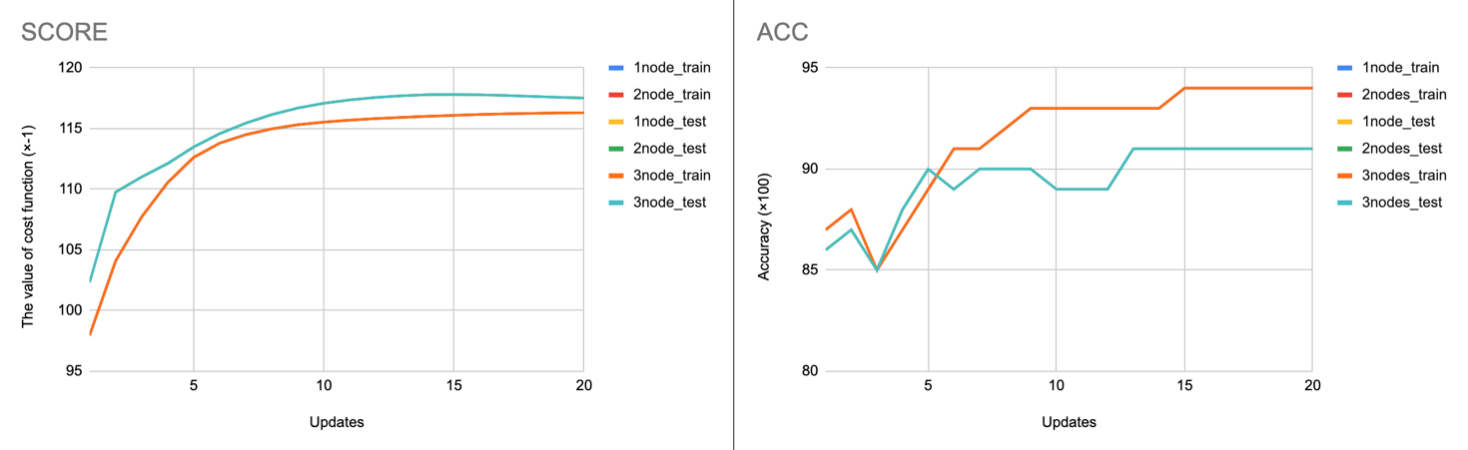
\includegraphics[keepaspectratio, scale=0.54]{experiment/figure/ignore_MNIST_node_change.png}
    \caption{MNIST classification with changed number of quantum node. Fixed at 6 qubits, 3 fraxis layers, 100 training and evaluation data. We ignored 5 decimal places of the matrix $G$.}
    \label{fig:ignore_MNIST_node_change}
\end{figure}

\par Figure \ref{fig:ignore_MNIST_node_change} shows exactly the same behavior of distributed algorithm from the non-distributed one.

%%%%%%%%%%%%%%%%%%%%%%%%%%%%%%%%%%%%%%%%%%%%%%%%%
%%%%%% conclusion
%%%%%%%%%%%%%%%%%%%%%%%%%%%%%%%%%%%%%%%%%%%%%%%%%

% 結論
\chapter{Conclusion \label{chap:conclusion}}
\section{Our contributions}
\par Our aim is to make full use of exsitent quantum resources for machine learning with big data. In order to handle big data, it is necessary for the speed of training the model to be fast for the data size. Although  variational method is faster than kernel method, it is not sufficient when handling big data. In order to speed up variational method, we want to parallelize variational method with multiple quantum processors.
Furthermore, it is better if there is no need to aggregate given data to the central server, because communication of big data is troublesome (quantum federated learning).
  
\par In this paper, we propose a new distributed coordinate descent algorithm for quantum classification. 

\par Our research has impacts like below:

\begin{enumerate}
\item Our algorithm uses gradient-free optimizer for quantum machine learning, especially for classification. Up until now, algorithms using gradient-free optimizers are mainly focused on optimization problems or chemistry (solving eigenvalue problems for ground state energy computation), not with machine learning. We invent a new algorithm to construct a cost function for quantum classification, which makes it possible to minimize the function gradient-freely.

\item Our algorithm can be parallelized despite using a gradient-free optimizer. Up until now, distributed algorithms were based on gradient-based optimizers\cite{Qi_2022, 9775600}. This is thought to be due to the fact that gradient-free optimizers have not been considered for distributed quantum machine learning algorithms until now because gradient-based optimizers are very associated with classical machine learning. We invent distributed quantum machine learning algorithm using gradient-free optimizers, which are said to converge faster than gradient-based algorithms. This parallelization method makes it possible to do large-scale machine learning using big data.

\item Our algorithm achieves linear-scale speed up in training by the degree of parallelization. This feature is proved theoretically and also indicated by numerical simulations.

\item Our distributed algorithm behaves almost the same as the non-distributed one. Theoretically both behaviors are proved to be completely equal, and numerical simulations support this feature to some extent. Since the recently proposed distributed algorithms use gradient-based optimizers, the results obtained will inevitably change depending on the degree of parallelism. This is the drawback in these distributed algorithms, but we use gradient-free optimizer and that makes it possible to obtain the same result as the non-distributed one.
 \end{enumerate}

\begin{figure}[htb]
    \centering
    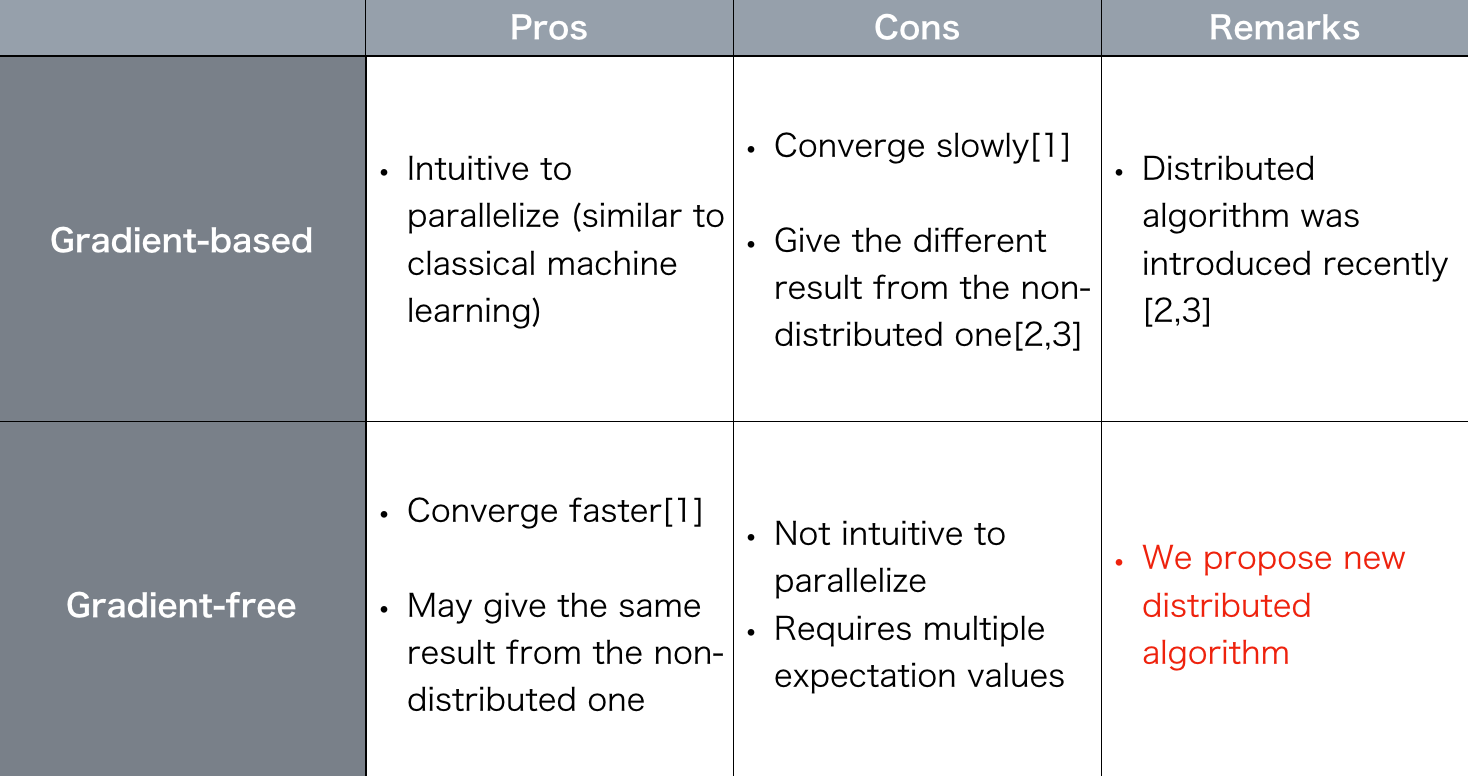
\includegraphics[keepaspectratio, scale=0.5]{introduction/optimizer.png}
    \caption{Our direction compared to the previous researches.}
    \label{fig:optimizer}
\end{figure}
\section{Future works}
While we reviewed our contributions above, many future works stem from this research. The issues obtained through these experiments are described below.

\subsection{Implementation on the real devices}
In our research, we did experiments of numerical simulation, but we did not do the experiments on the real devices. This is because the current Qiskit library does not have an API that realizes communication between multiple quantum computers and classical computers. One promising way to do experiments on the real device is to build multiple circuits on a single quantum computer. In our experiments of numerical simulation, we used qubits of the number from two to eight. The latest quantum computers have more than 100 qubits, so we can construct several quantum circuits at once on the single quantum computers. We would like to investigate how the effects of noise in quantum computers affect accuracy by experiments on the real device.

\subsection{Designing the cost function}

We designed the cost function like below:
$$-\sum_{i=1}^N y_{i}\tr{\left(Z_1 SR_d(\bm{n})Q\rho_{i} Q^\dagger R_d(\bm{n})^{\dagger}S^\dagger\right)}$$
Although the form of this cost function is very compatible with our optimization method, minimization of this function does not always improve the accuracy of the prediction, and sometimes even make it worse. One direction would be to devise a cost function that directly leads to improved accuracy while keeping the cost to optimize parameters low. This may lead to faster convergence.

\subsection{Circuits construction}

Coordinate algorithm iterates updating of the parameters one by one, therefore the order of the updating and the initialization of the parameters have a great influence on performance.
In our experiments of numerical simulation, we initialized the all fraxis gates' parameters to $bm{n}=(0,0,1)^\top$, and the order of updating of the parameters is cyclically fixed. Finding the new method to initialize the parameters and determine the order of updating may result in better performance. Furthermore, only one type of the ansatz (the pattern of gate replacement), one way of the encoding is tested in our research. There are many possible variations of quantum circuits construction along the lines of our research.
%%%%%%%%%%%%%%%%%%%%%%%%%%%%%%%%%%%%%%%%%%%%%%%%%
%%%%%% appendix
%%%%%%%%%%%%%%%%%%%%%%%%%%%%%%%%%%%%%%%%%%%%%%%%%

\newpage
% \appendix
\chapter{Appendix \label{chap:appendix}}
$$\begin{aligned}
\frac{\partial }{\partial x_k}\bm{x}^\top A\bm{x}&=\frac{\partial }{\partial x_k}\sum_{i}x_i(A\bm{x})_i\\
&=\frac{\partial }{\partial x_k}\sum_{i}x_i\sum_{j}A_{ij}x_{j}\\
&=\frac{\partial }{\partial x_k}\sum_{i}\sum_{j}A_{ij}x_{i}x_{j}\\
&=\sum_{i}\sum_{j}A_{ij}\frac{\partial }{\partial x_k}(x_{i}x_{j})\\
&=\sum_{i}\sum_{j}A_{ij}(\delta_{jk}x_{i}+\delta_{ik}x_{j})\\
&=\sum_{i}A_{ik}x_{i}+\sum_{j}A_{kj}x_{j}\\
&=(A^\top\bm{x})_{k}+(A\bm{x})_{k}\\
&=\left((A+A^\top)\bm{x}\right)_{k}
\end{aligned}$$
Therefore, 
$$\frac{\partial }{\partial \bm{x}}\bm{x}^\top A\bm{x}=(A+A^\top)\bm{x}$$
Here, 
$$\delta_{ij}=\begin{cases}
1 & \rm{if}\ i=j\\
0 & \rm{otherwise}\\
\end{cases}$$


%%%%%%%%%%%%%%%%%%%%%%%%%%%%%%%%%%%%%%%%%%%%%%%%%
%%%%%% references
%%%%%%%%%%%%%%%%%%%%%%%%%%%%%%%%%%%%%%%%%%%%%%%%%

%-------------------
\bibliographystyle{plain} % 参考文献
\bibliography{myref} %
%-------------------
\end{document}